\chapter{Requirements}

In the previous section, we have already identified some concepts that could also provide useful in a cross-device testing scenario. Those concepts include:
\begin{itemize}
	\item Emulation of multiple devices
	\item Easy integration of real and emulated devices
	\item Easy switching of device configurations
	\item Integration with Debugging Tools
	\item Automatic connection management
	\item Coordinated record and replay
\end{itemize}

While some of those concepts can be adopted without much adjustment, others still have some limitations that make them difficult to use for cross-device testing and need to be extended in some ways. Other concepts are completely new and targeted specifically at cross-device application testing. In the following sections, we will describe the key requirements for XDTools.

\section{Emulation of Multiple Devices}

Device emulation is already often used for testing responsive websites. In its simplest form, device emulation is just resizing a browser window so it looks and feels like a smaller device. However, manually resizing a browser window such that it has a resolution that is typical for actual devices is difficult. Furthermore, just emulating the screen size is not enough to realistically emulate a real device: Mobile devices typically use touch interactions and often have poor network connectivity. Those limitations have led to the emergence of more sophisticated tools for device emulation. Advanced device emulation facilities like the Device Mode in Chrome DevTools emulate different screen sizes, touch capabilities, network conditions, as well as location and acceleration sensors. They also typically provide a long list containing existing devices. However, all those tools have one common limitation: They can emulate only one device per browser tab or window. Another limitation of those tools is that even when multiple browser windows are used, those browser windows share the same local resources such as local and session storage. This limits the use of those tools for cross-device application testing, as cross-device applications typically run on multiple independent devices simultaneously and thus should not share any local resources. To accurately simulate the use of a cross-device application in real life, some mechanism for preventing devices from sharing local resources is required. There are several possibilities for doing this: First, multiple different browser profiles can be used. Second, the incognito mode provided by most browsers can be used to prevent sharing of local resources. Lastly, multiple independent browsers can be used. However, those solutions all have some limitations: Using multiple independent browsers obviously limits the number of devices that can be emulated to a rather small number. Also, all those solutions require multiple windows that need to be arranged somehow and tasks like creating multiple browser profiles are time-consuming and might not be what the developer wants. This is tedious and frequent switching between browser windows is required. Finally, not all browsers support multiple browser profiles, limiting the number of browsers on which an application can be tested. Additionally, if the developer actually wants to use browser debugging tools, those tools have to be opened in for each window separately which requires a lot of space and also limits the number of devices that can realistically be emulated. The screen size of the device that is used for emulating the devices can also be a limitation in other scenarios: If the device has a full HD screen but the developer wants to emulate a full HD device as well as some mobile devices simultaneously, those devices cannot be ordered such that all devices are visible at the same time. The developer would need to put one window in full screen and switch browser windows when they want to access the other devices. Constantly switching between devices can be tedious and the consequences of interactions performed on one device on other devices cannot be observed in real-time because switching between windows requires some time. Also, things like emulating a 4K TV on a full HD screen are even more difficult.

Those limitations all contribute significantly to the difficulty of cross-device application testing. Using these limitations, we gathered a number of requirements for device emulation in XDTools:
\begin{itemize}
	\item It should be possible to \emph{emulate multiple devices} in one browser window.
	\item The emulated devices should \emph{not share any local resources}.
	\item The screen size should not be a major limiting factor concerning the number of devices that can be emulated simultaneously. This can be realized by \emph{scaling devices} down without changing their resolution.
	\item The developer should have access to a list containing some \emph{existing devices}.
	\item The developer should be able to \emph{dynamically change the resolution}.
	\item The developer should be able to add and save \emph{custom devices}.
\end{itemize}

Scaling devices down while keeping the resolution and resizing devices are two different concepts. The difference between the two is illustrated in Figure~\ref{fig:difference_resizing_scaling}.

\begin{figure}[H]
  \centering
    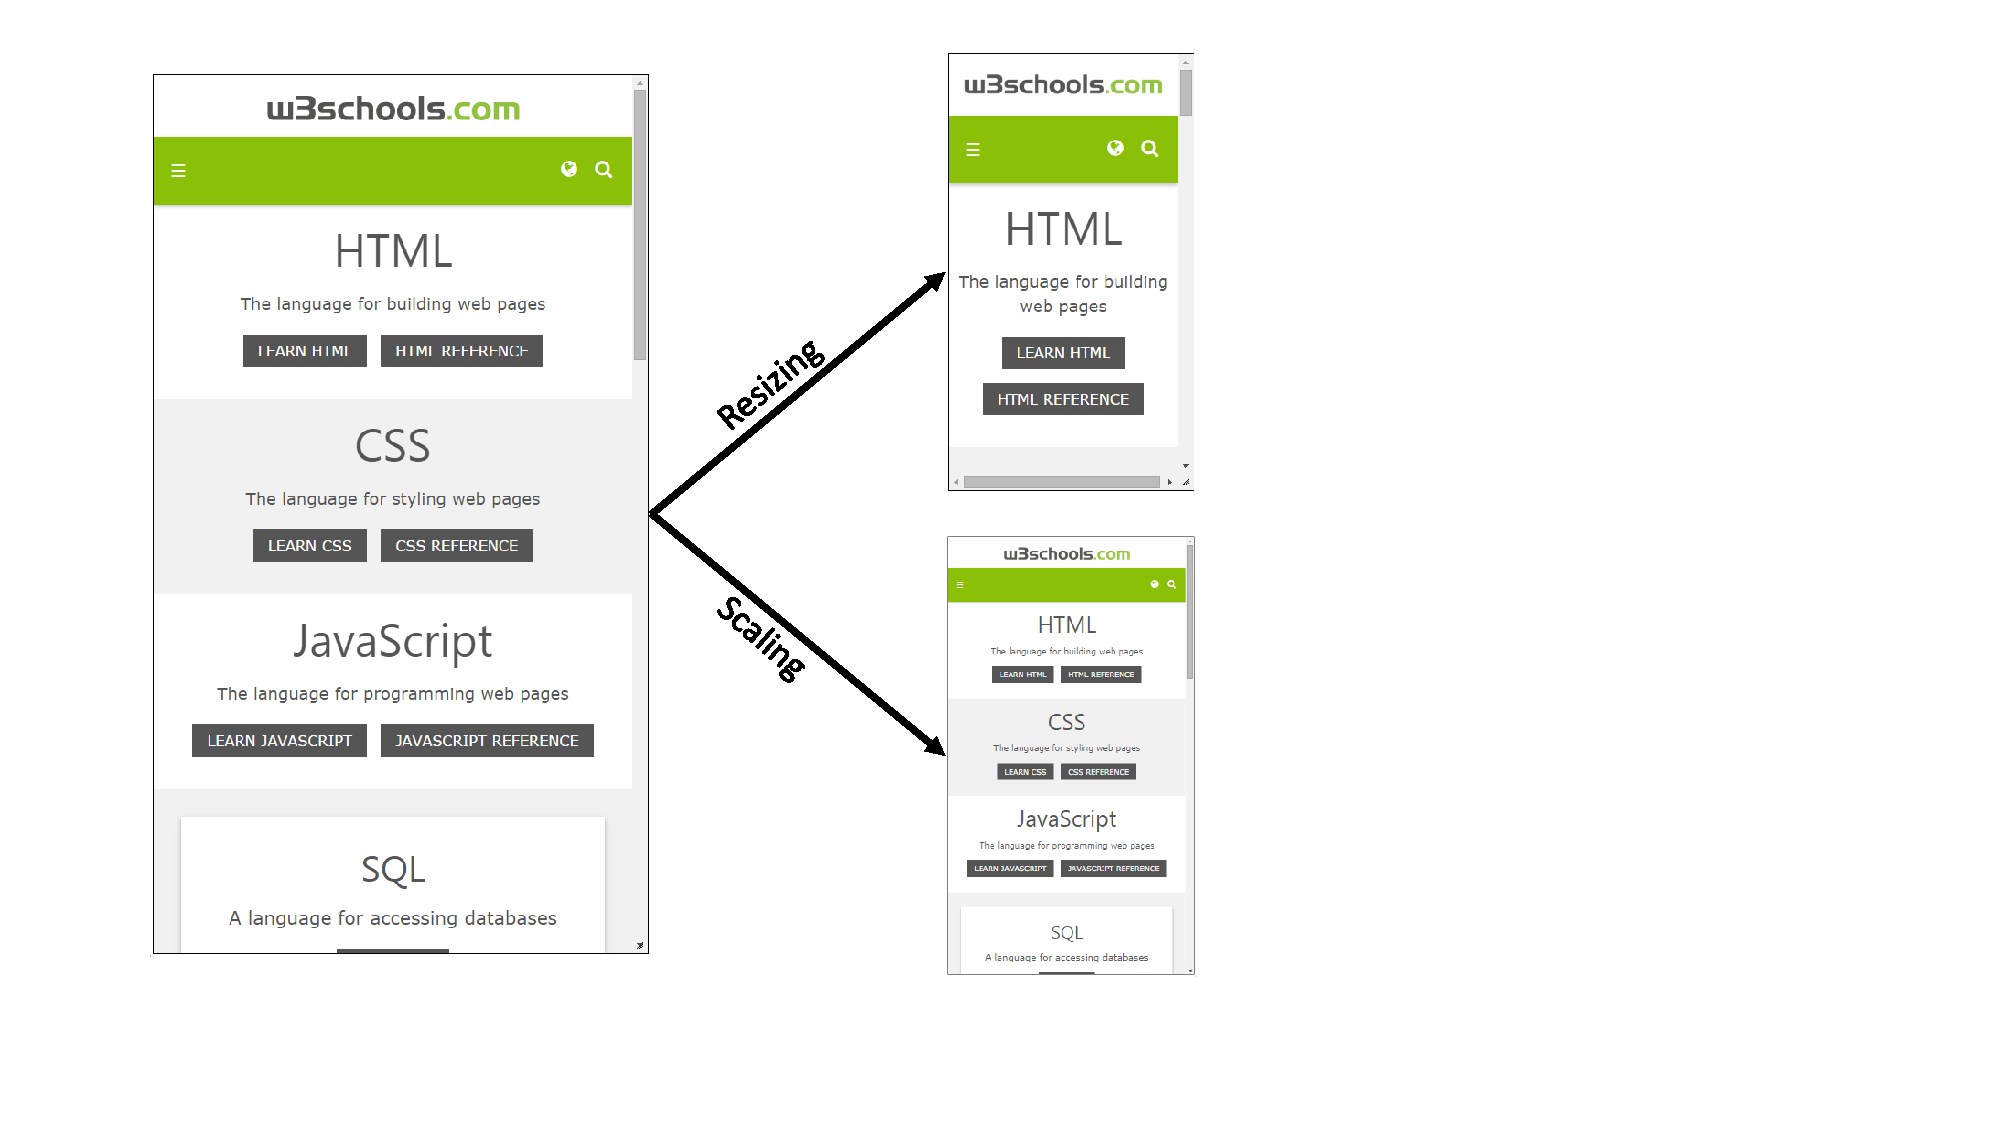
\includegraphics[width=1.0\textwidth]{images/difference_scaling_resizing.pdf}
	\caption[Difference between resizing and scaling a device]{Difference between resizing and scaling a device}
	\label{fig:difference_resizing_scaling}
\end{figure}

\section{Easy Integration of Real and Emulated Devices}

Emulating devices is a versatile tool for testing cross-device applications on many different devices. However, it does not completely eliminate the need for testing on real devices: Device emulation is always limited to certain aspects that are being emulated, e.g. screen size, resolution, touch interactions, location, and more. However, not every little detail of a real device can be emulated accurately. The following list provides an overview of some of the other limitations regarding testing on emulated devices only:
\begin{itemize}
	\item Touch interactions: Even though modern device emulators can also emulate touch interactions, performing a gesture with the mouse will never feel the same as the actual touch interaction. An interaction that works great with the mouse might feel awkward when performed on a real device and vice-versa. Also, multi-touch interactions such as pinching are difficult to emulate in a realistic way on an emulated device.
	\item Interrupts: While using an application on a real device, the user might be interrupted by things like the arriving of a text message. Those interrupts cannot be simulated in a realistic way on an emulated device.
	\item Performance: A desktop PC typically has much more computing power than a mobile device. If an application performs poorly on mobile devices, this might not even be noticed if the developer only tests on emulated devices.
	\item Display: The display quality and thus also the look of an application varies greatly depending on the device. Only emulating devices on a desktop PC cannot account for those differences in display quality. 
	\item Sensors: Modern devices have a large number of different sensors that cannot all be emulated realistically. One particular problem is the orientation of the device: A user might switch between landscape mode and portrait mode on purpose or accidentally at multiple points. Although the orientation of emulated devices can also be switched, this does not accurately simulate the behavior of a real user.
\end{itemize}
Although this list gives a good overview of the limitations of testing on emulated devices only, this list is by far not complete and what happens on a real device cannot always be foreseen by testing on emulated devices. Thus, testing on real devices is crucial for the successful development of a cross-device application. 

The importance of testing on real devices leads to a new requirement for XDTools: It should easily be possible to connect real devices to XDTools. 

\section{Easy Switching of Device Configurations}

Cross-device applications are typically used by different sets of users and thus also different devices. Even the same user may sometimes use their mobile phone and laptop simultaneously and at other times only their mobile phone or tablet. Thus, the number of devices being used with a cross-device application and those devices' characteristics may vary greatly. Depending on the devices connected to a cross-device application, the UI distribution might be different. A cross-device application needs to be able to support all those different device scenarios. However, some cross-device applications are also targeted to specific scenarios, e.g. a presentation room with multiple big screens that are always present, in addition to some mobile devices that are only in the room when their owner is attending a presentation. In such an application, the developer would probably want to emulate or connect the two static devices whenever they are testing the application and dynamically add some mobile devices. Thus, it is a key requirement for XDTools that multiple different device scenarios can quickly be created and switched to support testing a large number of different use cases for applications. 

\section{Integration with Debugging Tools}

Many of the features integrated into the debugging tools of browsers are also immensely useful for testing cross-device applications, and some might even help more when testing cross-device applications than when testing traditional web applications. However, those tools are typically limited to debugging one device at a time. We have established before that XDTools should allow emulating of multiple devices in the same browser window. While this already simplifies debugging of multiple devices simultaneously somewhat, it also introduces some additional difficulties. The messages that are logged from all emulated devices are all shown in the browser debugger tools of the same window. However, trying out some things in the console by sending commands to devices becomes more difficult. Google Chrome allows the developer to switch between different frames in the console and thus address different frames with commands, but it is not always obvious which frame corresponds to which device. Also, the developer might want to try out the same thing on multiple devices and would have to switch between multiple frames to address all devices. Furthermore, even though logging messages from all devices are displayed in the console, it is difficult to find out which device sent the message. This further complicates the debugging of cross-device applications. The same limitation applies to JavaScript errors that are shown in the console, but cannot easily be related to a device. Further limitations of the browser-included debugging tools include that navigating to the HTML of an emulated device can be rather tedious, that CSS can only be applied to one device at a time and that function breakpoints can only be added on one device at a time. Especially the last limitation can make cross-device application testing difficult because different devices have different responsibilities and not all devices might use all JavaScript functions. Consequently, adding a breakpoint inside a function on one device might not help with debugging the function at all, because the function is not even called on that device. The existence of real devices complicates things even more. By connecting the device to the desktop PC via cable, the developer gets access to remote debugging in Google Chrome. Remote debugging provides the same debugging tools as the normal debugging tools, but debugging multiple devices at the same time gets even more difficult. The remote debugging of each device is opened in a new window, thus the developer once again has to navigate between multiple windows. Also, getting an overview of all logging messages from all devices and sending commands to multiple devices becomes even more difficult. However, integrating existing debugging tools into XDTools is clearly desirable: Most of those tools have been around for quite some time and thus are already well tested and have gone through a series of improvements. Also, almost all web developers have already used those tools for extensive testing and are thus already familiar with them. However, XDTools needs to extend those tools to support debugging on multiple devices simultaneously. From all this information, we derived the following requirements for XDTools:
\begin{itemize}
	\item Logging messages should all be aggregated in one place and the device the messages originated from should be easy to identify.
	\item JavaScript errors should also be aggregated and easily identifiable.
	\item It should be possible to send JavaScript commands to multiple devices at a time. 
	\item It should be easy to inspect the HTML of a specific device.
	\item It should be possible to add CSS to multiple devices at the same time (see Figure~\ref{fig:css_aggregation}).
	\item It should be possible to add breakpoints to multiple devices simultaneously.
	\item If possible, all of the above requirements should be applied to both real and emulated devices.
\end{itemize}

\begin{figure}[H]
  \centering
    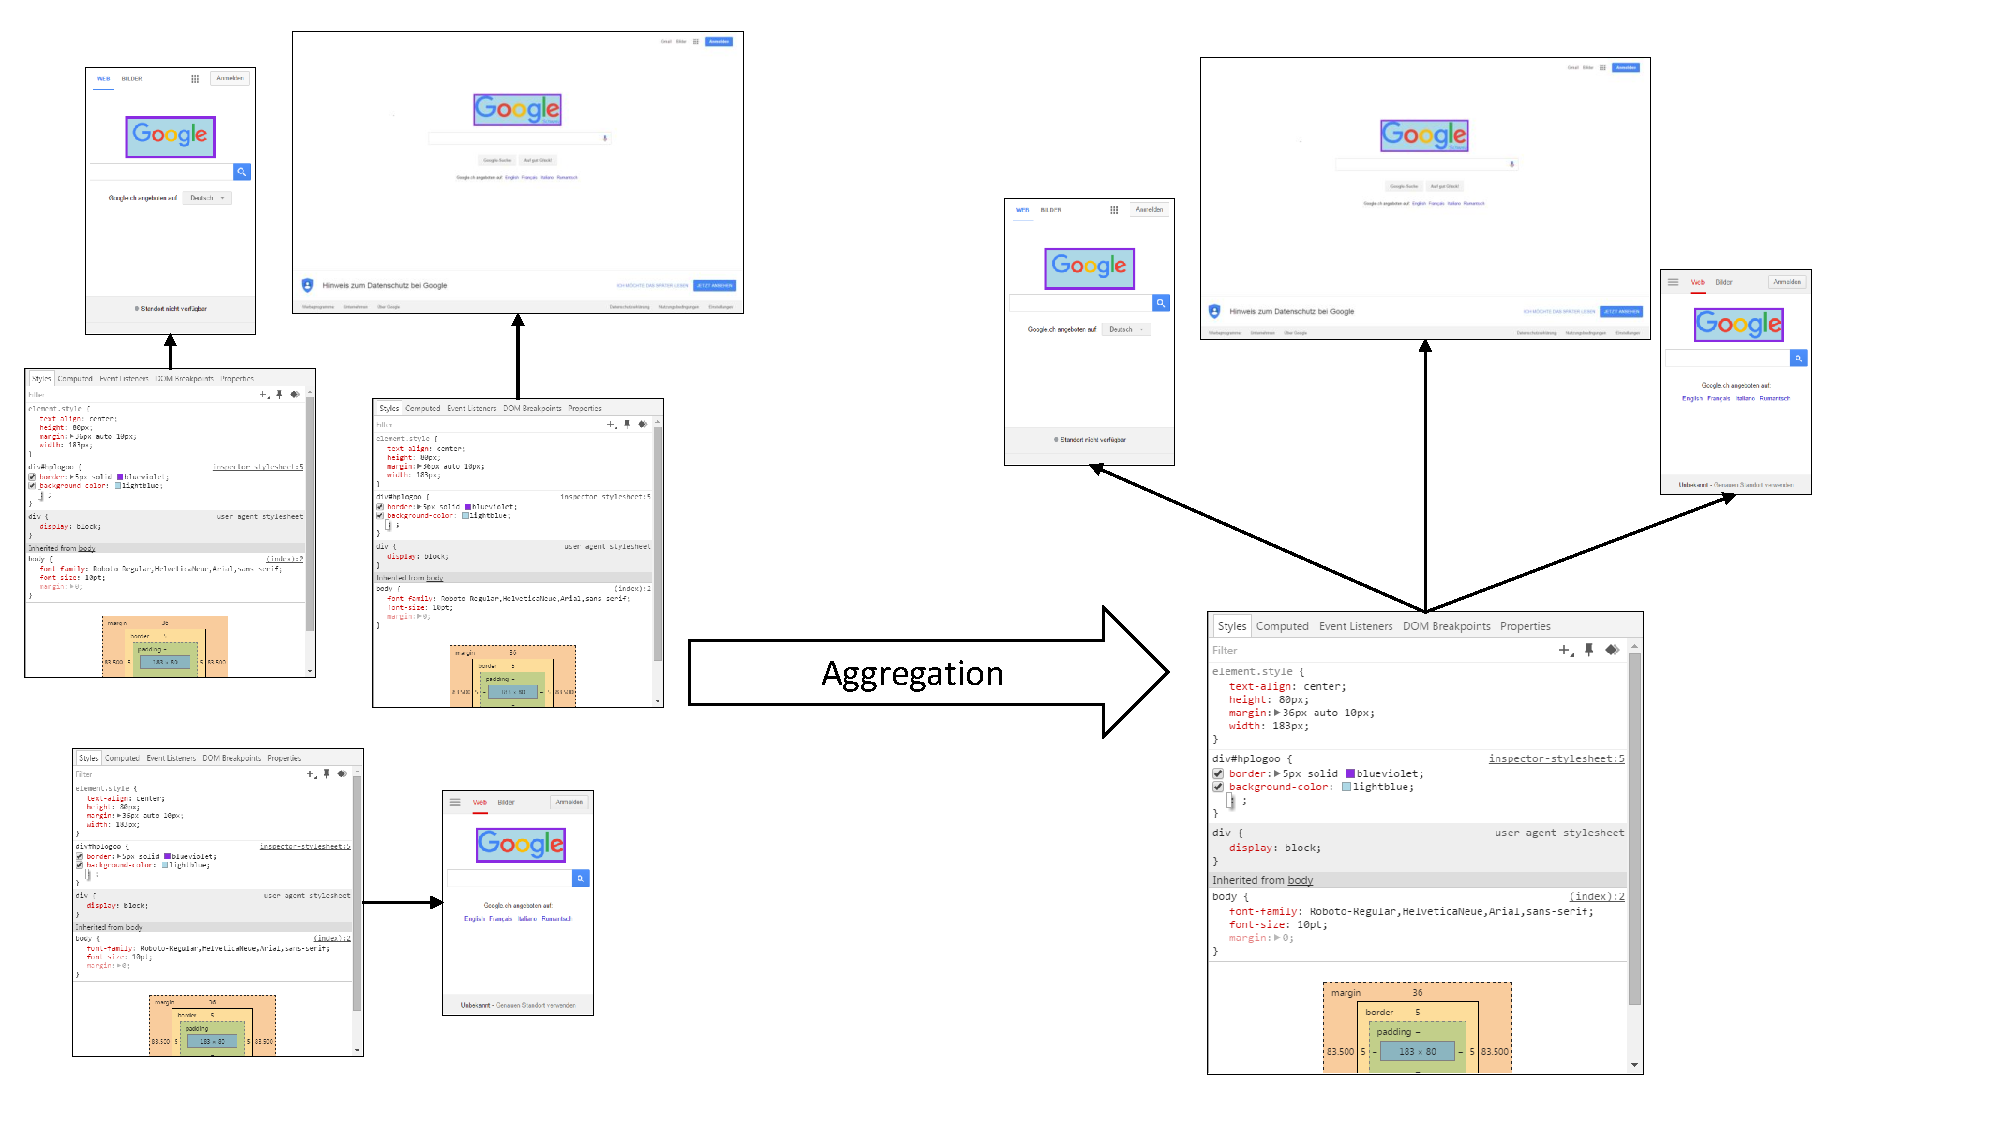
\includegraphics[width=1.0\textwidth]{images/css_aggregation.pdf}
	\caption[CSS editor aggregation]{CSS editor aggregation}
	\label{fig:css_aggregation}
\end{figure}

\section{Automatic Connection Management}

In order to use multiple devices in a cross-device application, those devices need to be paired with each other in some way. The mechanisms for pairing devices differ between different cross-device application frameworks: With some frameworks, all devices that open the cross-device application are paired implicitly. In other frameworks, for example XD-MVC, devices can be paired by copying the URL from one device to the other devices that should be connected. Other frameworks have more complicated mechanisms for connecting devices. In Connichiwa, one device runs a local web server and uses Bluetooth to detect nearby devices. The device then sends the IP of the web server over Bluetooth, enabling the other devices to access the received IP in a web browser. All of those three mechanisms have one thing in common: Devices are connected by opening a specific URL in the browser. However, other ways of connecting devices are also feasible: Some frameworks provide a function that can be called from a device to connect the device to another device by passing the ID of the device the device should be connected to. Also, many of the papers describing cross-device application development frameworks do not describe how devices are connected. Finally, cross-device applications can also be implemented independently of any framework and might use even more different ways for connecting devices. Thus, it is impossible to derive all ways in which devices could be connected in a cross-device application.

However, if the developer wants to debug a cross-device application, re-connecting the devices every time a new device configuration is used or possibly even when devices are refreshed is tedious and time-consuming. Thus, it is desirable to have some easy way of connecting devices. From this, we derive the next requirement for XDTools: It should be possible to automatically and manually connect devices to each other.

\section{Coordinated Record and Replay}

Record and replay has already been used previously for recording and replaying user interactions in traditional web applications and especially AJAX web applications. The non-deterministic and asynchronous nature of web applications contributes much to the value of recording and replaying interactions in web applications. When a bug is encountered during web application testing, it is often difficult to determine the exact steps for reproducing the bug. Reproducing bugs becomes even more difficult in cross-device scenarios where multiple devices are involved and the interactions performed on one device have some implications on other devices as well. Also, cross-device applications are often used by multiple users at the same time and it is difficult for the developer to simulate multiple users interacting with their devices simultaneously. Thus, we believe that record and replay can benefit cross-device application developers even more than developers of traditional web applications. However, precise mechanisms for timing replay are needed if we want to simulate multiple users simultaneously. Also, simply replaying interactions is not enough: If something goes wrong during an interaction, we need some way of pausing the replay and inspecting the state of the devices. XDTools should implement a record and replay mechanism that fulfills the following requirements:
\begin{itemize}
	\item All interactions with the device should be recorded. 
	\item It should be possible to replay a sequence of interactions on another device than the device that recorded the sequence.
	\item It should be possible to pause the replaying of the interaction sequence.
	\item Accurate timing of replays should be possible.
\end{itemize}